%----------------------------------------------------------------------------   
\chapter{Használt eszközök bemutatása}
%---------------------------------------------------------------------------- 

\section{Médiasík protokollok}

\subsection{RTP \& RTCP}

Az RTP protokoll használatával valós időben lehet hang, videó vagy egyéb multimédiás 
információkat szállítani egy-egy felhasználó között. A valós idejű továbbítás mellett
információkat szolgáltat arról, hogy a csomag tartalma milyen kódolást használ, 
sorszámozza a csomagokat, ellátja őket időbélyeggel és lehetővé teszi a szállítási 
folyamat monitorozását. Az alkalmazások általában UDP felett használják az RTP-t 
\cite{RFC3550}, mivel az UDP a TCP-vel (Transmission Control Protocol) ellentétben nem 
tartalmaz folyam- és torlódásvezérlést illetve automatikus hibajavítást, ezért jobban 
illeszkedik a médiaátvitel valós-idejű követelményeihez. Ez viszont nem azt jelenti, hogy 
az RTP csak UDP-vel tud működni, mert elméletileg minden UDP-hez hasonló protokoll tudja 
kezelni az RTP-t \cite{RFC3550}.

Fontos megjegyezni, hogy az RTP nem szolgáltat semmilyen mechanizmust, ami biztosítaná,
hogy a csomagok időben megérkeznek és így QoS-t (Quality of Service) sem garantál. 
Ezenkívül az RTP nem garantálja, hogy a csomagok egyáltalán megérkeznek, nem akadályozza 
meg, hogy a csomag soron kívül érkezzenek és nem ellenőrzi, hogy a használt hálózat 
megbízható és az sorban szállítja le csomagokat \cite{RFC3550}. A fogadó alkalmazás 
feladata, hogy csomagokat sorba rendezze a bennük megtalálható sorszám alapján.

Ahhoz, hogy bővebb információt lehessen kapni az RTP folyam állapotáról periodikusan a 
felek küldenek egymásnak RTCP csomagokat. Ezek a csomagok szintén UDP felett működnek,
mivel ugyanazokra a funkcionalitásokra van szükség ebben az esetben is. Fontos megjegyezni
még azt is, hogy az RTP csomagok mindig páros portra érkeznek, míg az RTCP mindig az eggyel nagyobb portot fogja használni így az mindig páratlan lesz.

Fontos, hogy az RTCP csomagoknak számunkra két fő típusa van, amiket jelentéseknek hívnak.
Ezek a jelentések tartalmazzák az aktuális RTP folyamról alkotott információk halmazát. 
Ilyen jelentéseket a küldő és fogadó fél is készít. Viszont ez a kettő jelentés 
nem azonos mezőket tartalmaznak, mert a fogadó jelentésben számításba van véve a küldő 
jelentéseknek a tartalma és ideje. Ezeket a jelentéseket a hívásban résztvevő felek 
mindegyike periodikusan állít elő. Ez a periodicitás attól függ, hogy a hálózat mekkora 
sávszélességgel rendelkezik, ha nagyobb a sávszélesség, akkor több jelentés fog születni 
és jobb képet lehet kapni arról, hogy milyen RTP folyam minősége, míg alacsonyabbnál 
kevesebb RTCP csomag kerül kiküldésre. 

A \cite{RFC3550} leírásában szereplő RTCP csomagok leírása alapján a fontosabb részei a
küldő és fogadó jelentésnek. Kezdve a küldőével: 

\begin{itemize}
	\item SSRC (Synchronization source), amivel jelöli, hogy kitől származik egy a 
	jelentés.
	\item A jelentés küldésének idejét, ami a küldő órájának pontos ideje. Körülfordulási
	idő mérésére használható. 
	\item RTP csomagokban használt időbélyeg. 
	\item A küldő által elküldött csomagok száma és azok mérete.
\end{itemize}

Míg a fogadó jelentés az alábbi részekkel rendelkezik:

\begin{itemize}
	\item SSRC.
	\item Töredékveszteség, ami az előző küldő és fogadó jelentés óta elvesztett RTP 
	csomagok számával van jelölve.
	\item Az összes elveszett csomag száma. 
	\item Legmagasabb kapott sorszám. 
	\item A csomag küldési időpontjától az érkezés idejéig eltelt idő, ami a Jitter. Ez 
	az érték minden fogadó jelentés során újra van számolva a két jelentés között 
	érkezett csomagok alapján.
	\item Az utolsó kapott küldő jelentés ideje és az azóta eltelt idő.  
\end{itemize}

\subsection{SIP}

A SIP egy olyan alkalmazásrétegben működő viszonykezdeményező protokoll, amivel 
létrehozni, módosítani és törölni lehet kapcsolatokat felek között. Ezek a kapcsolatok 
általában az internet telefonálás vagy multimédiás forgalom lebonyolítását valósítják meg. 

A SIP működése során fontos, hogy a felhasználók azonosíthatóak legyenek valamilyen
paraméter szerint, amihez sok esetben nem elegendő szimplán az IP cím. Egy 
SIP kliens egyéniségét a SIP URI (Uniform Resource Identifier) fogja megadni, ami
a  felhasználó nevéből és a SIP szerver által meghatározott tartománynévből áll.
Ez a cím úgy néz ki, mint egy átlagos email cím azzal a különbséggel, hogy az 
elején szerepel a \texttt{sip:} szó. Egy példa arra, hogyan néz ki egy ilyen cím: 
\texttt{sip:peter@tartomany.com}. Így ha az egyik kliens hívást kezdeményez Péter felé,
akkor ezzel a címmel pontosan meglehet határozni az elhelyezkedését. 

Működése nagyban hasonlít a HTTP (HyperText Transfer Protocol) kommunikációhoz, ahol 
a kliens bizonyos kéréseket küld a szerver felé, amire választ kap. A \cite{RFC3261} 
leírásban olvasható több parancs közül a szakdolgozat szempontjából a következők 
fontosabbak: 

\begin{itemize}
	\item \textbf{INVITE}: Új kapcsolat létesítése.
	\item \textbf{ACK}: INVITE üzenet elfogadását jelzi. 
	\item \textbf{BYE}: Kapcsolat befejezése. 
	\item \textbf{REGISTER}: Felhasználó regisztrálása a SIP szerverre. 
\end{itemize}

A SIP protokoll szerves része a multimédia folyamatok kiépítésénél szükséges SDP (Session 
Description Protocol). Az SDP leírókkal meg lehet adni, hogy a hívásban résztvevő felek 
milyen médiakódolásokat támogatnak és mely portokon várják a médiaforgalmat. Ezeken az 
információkon kívül még rengeteg más hasznos információt is lehet közölni ezekben az 
üzenetekben, viszont a szakdolgozat szempontjából csak a támogatott kódolás és a 
kapcsolat leírására szolgáló paraméter a fontos.

\section{Kubernetes}\label{sec:kubernetes}

A Kubernetes egy nyílt forráskódú konténer kezelő platform, amivel automatizálni
lehet a legtöbb feladatot, ami a fejlesztés, karbantartás vagy skálázással 
kapcsolatos. A Google fejlesztette eredetileg, de jelenleg a Cloud Native
Computing Foundation - CNCF vette át a karbantartását. 

Kubernetes fürtöt létrehozhatunk lokálisan saját szerveren is vagy felhőben,
ami lehet publikus, privát vagy hibrid hozzáférésű. Viszont azt figyelembe 
kell venni, hogy egy Kubernetes fürtöt nem egyszerű kiépíteni lokálisan, 
szóval ha nem szükséges, akkor lehet használni a felhőszolgáltatók Kubernetes 
motorjait, mint az Amazon AKS, Linode LKE vagy a Google GKE szolgáltatása.
Ilyenkor az általunk beállított paraméterekkel létrejön egy teljes klaszter, amit
tudunk menedzselni.

\subsection{Felépítése}

\begin{figure}[!ht]
	\centering
	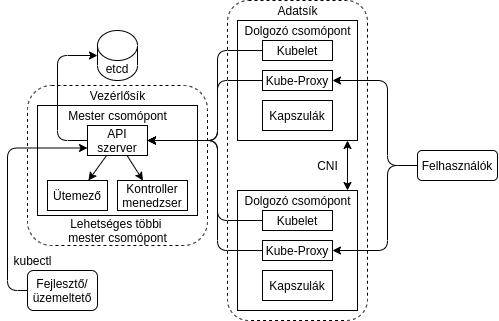
\includegraphics[width=1\textwidth, keepaspectratio]{figures/k8s_architecture.png}
	\caption{Kubernetes klaszter felépítése}
	\label{fig:achitecture}
\end{figure}

Egy Kubernetes fürt kettő részből áll egy vezérlő- és egy adatsíkból, ahol a 
vezérlősíkban szereplő mester csomópontok tudják vezérleni az adatsíkban 
lévő dolgozó csomópontokat és a fejlesztők vagy üzemeltetők a mester által
hirdetett API-n (Application Programming Interface) keresztül képesek parancsokat
kiadni. Míg a dolgozó csomópontokon futó alkalmazáshoz a felhasználók csak az 
általuk hirdetett Kube-Proxy segítségével tudnak hozzáférni. 

A kapcsolat mester és dolgozó között az API szerver és a Kubelet kommunikációján
alapul. Ha a fejlesztő szeretne egy új alkalmazást telepíteni a klaszteren, akkor
szól az API szervernek, ami majd kiadja a megfelelő parancsokat a Kubelet-nek 
és majd az fogja a konténereket létrehozni.

\subsubsection{Vezérlősík}

A mester csomópont mindig a fő vezérlő egysége a klaszternek, mivel kezeli a 
munkafolyamatokat és irányítja a kommunikációt klaszteren belül. A 
\ref{fig:achitecture}-s ábrán látható vezérlősík tartalmazhat több mester csomópontot is 
a felsorolt komponensekkel, amivel lehet biztosítani a fejlesztők számára a folytonos 
elérést. A mester csomópont részei: 

\begin{itemize}
	\item \textbf{etcd}: Egy állandó kulcs-érték alapú adatbázis, ami tárolja 
	a klaszter konfigurációs beállításait és a klaszter állapotát. Fontos az a rész, 
	hogy ez egy állandó adatbázis, mivel ez a csomóponton fut és nem egy 
	kapszulában.   
	\item \textbf{API szerver}: Egy REST API (Representational State Transfer API) 
	szerver, ami hozzáférést biztosít a klaszterhez a klaszteren belül és azon kívül is. 
	Egyszerű HTTP üzenetekbe ágyazott JSON (JavaScript Object Notation) konfigurációkkal
	lehet beállítani, hogy mit csináljon a klaszterben. De a dolgozó csomópontok is ezen 
	keresztül küldenek frissítést az etcd-be. 
	\item \textbf{Ütemező}: Ez a komponens dönti el, hogy egy új kapszula melyik
	dolgozó csomóponton legyen létrehozva aszerint, hogy van-e megfelelő erőforrás
	az adott csomópontot megvalósító szerveren.
	\item \textbf{Kontroller menedzser}: Egy olyan állandóan futó folyamat, ami ellenőrzi,
	hogy a kapszulák bizonyos esetekben újrainduljanak vagy hogy egy ismétlődő 
	munkafolyamat időnénként lefusson helyesen. Ezt az API szerverrel kommunikálva
	képes megvalósítani. 
\end{itemize}

A \ref{fig:achitecture} ábrán látható, \texttt{kubectl} eszköz segítségével a fejlesztők 
és üzemeltetők képesek kommunikálni az API szerverrel. Ez az eszköz lényegében
megvalósítja a teljes HTTP kommunikációt az API szerverrel szóval sokkal könnyebben 
lehet vele lekérdezni információkat vagy új erőforrásokat létrehozni. 

\subsubsection{Adatsík}

Az adatsíkon futnak az úgynevezett dolgozók, amik igazából különálló szerverek,
amik rendelkeznek a \ref{fig:achitecture}-s ábrán szereplő komponensekkel és képesek 
futtatni valamilyen konténer kezelő alakalmázást, például Docker-t. Régebben a Docker
alapértelmezett konténer kezelője volt a Kubernetes-nek, de 2021-ben már nem követeli meg 
és bármilyen másik konténer kezelőt is be lehet állítani alapértelmezettnek. A fontosabb 
elemei az adatsíknak:

\begin{itemize}
	\item \textbf{Kubelet}: Felelős az egyes csomópontok futási állapotáért biztosítva, 
	hogy a csomóponton lévő összes konténer egészséges legyen. Gondoskodik az alkalmazás
	konténereinek indításáról, leállításáról és karbantartásáról, amelyek kapszulákba 
	vannak rendezve a vezérlősík utasítása szerint
	\item \textbf{Kube-Proxy}: Egy proxy és terheléselosztó megvalósítása, ami biztosítja
	a szolgáltatás elérhetőségét más hálózatok számára. Feladata, hogy a beérkező
	forgalmat a megfelelő konténerekhez irányítsa, amit különböző paraméterek szerint 
	képes megvalósítani.
	\item \textbf{Kapszulák}: A legkisebb menedzselhető egységek, amiket lehet telepíteni
	Kubernetes alatt. Egy kapszula több konténernek a csoportja, amik osztoznak a tárolási
	és hálózati erőforrásokon és specifikálja, hogy a konténerek hogyan fussanak. 
	\item \textbf{CNI (Container Network Interface)}: A kapszulák hálózati interfészeinek
	a beállítására lehet használni. Segítségével specifikálni lehet, hogy a kapszulák között milyen hálózatot használva legyen továbbítva a forgalom. 
\end{itemize}

\subsection{Erőforrások}

A \ref{fig:achitecture} architektúra csak a fő erőforrásokat mutatja be, amiken kívül
még rengeteg olyan erőforrással is rendelkezik, amik lehetővé teszik a konténerek 
menedzselésének egy új szintjét. 

Ismertetem, hogy a projekt szempontjából mely erőforrások lesznek még lényegesebbek. 
Viszont rengeteg olyan erőforrásról lehet többet olvasni \cite{kubeAPI}, amiket a 
Kubernetes segítségével lehet létrehozni.   

\begin{itemize}
	\item \textbf{Replikációs vezérlő}: Biztosítja, hogy egy meghatározott számú 
	kapszula replika fusson egyszerre, amivel biztosítja az alkalmazás magas szintű
	elérhetőségét. Ezáltal, ha túl sok kapszula fut, amikre nincs szükség, 
	akkor a felesleges kapszulák törlésre kerülnek, míg abban az esetben, ha az elvártnál
	kevesebb kapszula érhető el akkor újakat hoz létre. Mindazonáltal, ha egy kapszula 
	maga vagy az egyik konténere hibát eredményez, akkor újraindítja a benne lévő 
	konténer vagy a teljes kapszulát. 
	\item \textbf{Telepítő (Deployment}): Leír egy elvárt állapotot, ami alapján a
	replikációs vezérlő tudja, hogy milyen specifikáció szerint kell az új kapszulákat
	létrehozni vagy a létrehozandó kapszulák számát. 
	\item \textbf{DaemonSet}: Biztosítja, hogy az összes vagy néhány csomópont 
	futtassa egy meghatározott kapszula másolatát. Ezáltal, ha egy új dolgozó csomópont 
	csatlakozik a klaszterhez, akkor ez a kapszula automatikusan megjelenik rajta. 
	Tipikusan valamilyen tárolási vagy monitorozási feladatot ellátó kapszulát szokás 
	ilyen módon létrehozni, de a későbbiekben látni fogjuk, hogy az L7mp ugyan ezzel a 
	módszerrel hozza létre a bejárati pontokat a csomópontokon.
	\item \textbf{DNS (Domain Name System)}: Tárolja a klaszterben szereplő minden 
	kapszula és szolgáltatás IP címét illetve a hozzájuk kapcsolódó tartomány nevüket 
	is.  
	\item \textbf{Szolgáltatás}: Egy absztrakt módja az alkalmazást futtató kapszulák
	kiexponálásának a hálózaton keresztül. Mivel a kapszulák halandóak így nem mindig
	ugyanazon a címen lesznek elérhetőek a rajtuk futtatott alkalmazások. A megoldás
	erre, ha egy címke alapján hozzárendeljük őket egy szolgáltatáshoz, ami mindig 
	elérhető lesz ugyanazon a címen és képes elosztani a forgalmat több kapszula között.
	A forgalomirányítást a szolgáltatások a Kubernetes DNS szolgáltatása miatt tudják 
	megvalósítani. Mivel minden kapszula rendelkezik egy tartománynévvel és ez a 
	Kubernetes DNS leírójában szerepel egy hozzá tartozó IP címmel.
	\item \textbf{Bejárat (Ingress gateway)}: Egy olyan API objektum, ami kezeli a 
	külső hozzáférést különböző szolgáltatásokhoz a klaszteren belül. Ezáltal a bejövő 
	forgalmat könnyen lehet szűrni illetve típusától, tartalmától függően más és más 
	szolgáltatásokhoz lehet irányítani. 
	\item \textbf{Egyéni erőforrás definíció (Custorm Resource Definition)}: A 
	Kubernetes API egy olyan kiterjesztése melynek során új fajta erőforrás definíciókat
	lehet definiálni, amik bővítik a Kurbenetes funkcionalitását.
	\item \textbf{Pótkocsi (Sidecar)}: Mivel egy kapszula több konténert is tartalmazhat
	és ezek a konténerek megosztják a hálózatukat így létre lehet hozni egy olyan 
	konténert, ami csak a hálózati forgalom kezelésével foglalkozik. Segítségévével lehet 
	szűrni, hogy milyen forgalom juthat csak el az alkalmazást futtató konténerhez. Mivel 
	elsőnek  mindig ezen pótkocsin fog áthaladni a forgalom majd lokális hálózaton átadja 
	az alkalmazásnak. Ezek a pótkocsik általában valamilyen proxyk szoktak lenni. 
	\item \textbf{RBAC (Role-based access controll)}: Ha több fejlesztő vagy üzemeltető
	fér hozzá az API szerverhez, akkor egyénenként meglehet mondani, hogy kinek milyen 
	művelet végrehajtására van joga. Például korlátozható, hogy ki képes új
	erőforrásokat létrehozni. Viszont a felhasználók mögött sokszor nem egy élő 
	személy van, hanem egy alkalmazáshoz van hozzárendelve. Ezáltal az alkalmazás 
	esetlegesen képes a klaszteren belülről erőforrásokat kezelni.
	\item \textbf{Operátor}: Olyan bővítések, amikkel egyéni erőforrások menedzselése
	valósítható meg. De emellett különböző eseményeknél lehet bizonyos folyamatokat 
	elindítani. Példának okáért, ha egy kapszula létrejön, akkor beállíthatjuk, hogy
	rendelkezzen mindig egy adott címkével.
	\item \textbf{Szolgáltatásháló (Service Mesh)}: Meghatározza, hogy a klaszter 
	különböző részei hogyan kommunikáljanak egymással. Ezt általában a pótkocsikkal és 
	egy operátorral valósítják meg. A pótkocsik fognak rendelkezni azokkal a 
	beállításokkal, hogy a mellettük futó konténer milyen forgalmat fogadhat és az 
	operátor fog arról gondoskodni, hogy a résztvevő kapszulák pótkocsijai mindig a 
	megfelelő beállításokkal jöjjenek létre.
\end{itemize}

\section{L7mp}

Az L7mp egy kísérleti alkalmazásréteg és több protokollt támogató szolgáltatás- proxy és 
háló keretrendszer. A hangsúly a több protokoll támogatásán van, amely lehetővé teszi, 
hogy sok szállítási- és alkalmazásréteg béli protokollt natívan támogasson és ne csak a 
szokásos TCP/HTTP protokollokat. Lehetővé teszik emellett még a protokollok közötti 
konvertálást is, amivel könnyen lehet alkalmazási rétegű protokollokat konvertálni 
szállításiba és vissza is.

Az L7mp egy vezérlő- és adatsíkból áll: az adatsíkot az L7mp proxy valósítja meg, míg a 
vezérlőt egy operátor, ami kezeli az L7mp proxy példányokat.

Ha egy másik szoftverhez kellene hasonlítani az L7mp-t, akkor leginkább az Istio-hoz 
lehetne, hiszen felépítésében nagyon hasonló elemeket használ, mint az Istio. Szóval 
akinek van valamilyen tapasztalata az Istio-val az könnyen kiismeri magát az L7mp-vel is.

Szeretném megemlíteni, hogy Dr. Rétvári Gábor vezetésével a nyári gyakorlati időm alatt 
és jelenlegi munkámként ennek a szoftvernek a tesztelésével  illetve fejlesztésével 
foglalkozom. Az L7mp már szerepelt a ServiceMeshCon 2020-s konferenciáján 
\cite{servicemeshcon_2020}, ahol Gábor bemutatta az L7mp szolgáltatásháló által nyújtott 
lehetőségeket. 

\subsection{L7mp, mint proxy}

Az L7mp proxy egy olyan programozható proxy, ami nagyon hasonlóan működik, mint az Envoy, 
ami egy széleskörűen használt leginkább alkalmazási réteget támogató proxy. A különbség 
az L7mp proxy és az Envoy között, hogy az L7mp proxy a szállítási réteg protokolljait  
támogatja jobban míg az Envoy inkább az alkalmazásréteg protokolljait képes jobban  
kezelni.Emellett az L7mp proxy képes protokollok közötti átalakítást végezni, ami sok 
esetben hasznos lehet. Ez a funkcionalitás az architektúra leírása után fog jobban 
megmutatkozni.

A L7mp proxy egy magas szintű keretrendszerben íródott, ezért nagyon egyszerűen 
lehet új funkciókkal bővíteni. Ez a keretrendszer a Node.js, ami egy JavaScript
futtató környezet a Google Chrome V8-s JavaScript motorjára építve. Ez szerencsés 
választás a már említett egyszerű bővíthetőség miatt, de amiatt is, hogy
könnyen lehet vele aszinkron módon programozni. Mivel nincsenek blokkoló műveletek,
amiket külön szálon kellene futtatni. De behozza azt a hátrányt is, hogy a 
JavaScript miatt lassabb az L7mp, mint az Envoy, ami C++-ban van írva. 

A lassúság kiküszöbölésére jelenleg vannak munkálatok, amik elsősorban azt 
célozzák meg hogy a csomagok feldolgozása nem a felhasználói névtérben kerüljenek
végrehajtásra, hanem kernel szinten. 

Az L7mp proxy használható szimplán Node.js-sel indítva, mivel elérhető az NPM (Node 
Package Manager) tárolóban. Az indítása a \ref{lst:nodeL7mp} paranccsal történik: 

\begin{lstlisting}[caption=L7mp indítása Node.js segítségével, label=lst:nodeL7mp]
node l7mp-proxy.js -c config/l7mp-minimal.yaml -l warn -s
\end{lstlisting}

A \ref{lst:nodeL7mp} parancs kiadása után a minimális L7mp konfigurációval és a 
figyelmeztetés naplózási szinten fog elindulni az L7mp proxy. A minimális konfiguráció 
létre fog hozni egy REST API szervert, amin keresztül a későbbiekben újabb L7mp 
beállításokat lehet megadni.

Ezen felül a Docker-t is támogatja, ami alapértelmezetten a \ref{lst:nodeL7mp} parancsot 
fogja egy konténerben futtatni.

\subsubsection{Felépítés}

Mivel az L7mp proxy tervezése során az Envoy volt a minta, így főbb elemei között 
szerepelnek ugyanolyan vagy hasonló elemek. 

\begin{figure}[!ht]
	\centering
	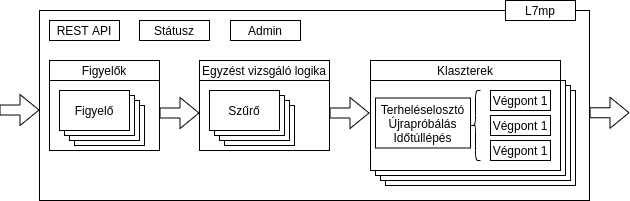
\includegraphics[width=1\textwidth, keepaspectratio]{figures/l7mp_struct.png}
	\caption{L7mp felépítése}
	\label{fig:l7mpStruct}
\end{figure}

A \ref{fig:l7mpStruct} ábrán látható, hogy az L7mp proxyn miképp vannak az elemek kapcsolatban egymással. A figyelők azok az erőforrások, amik elsőként kapják meg az L7mp proxyhoz beérkező csomagokat, majd ezeket a definiált szabályok alapján eljuttatja az L7mp klaszterekig, ahol a csomagok képesek eljutni a definiált végpontokig. 

Az alábbi felsorolás tartalmazza az L7mp proxy által használt erőforrások ismertetését.

\begin{itemize}
	\item \textbf{Munkamenet (Session)}: Munkameneteket nem lehet manuálisan létrehozni,
	mivel ezek akkor generálódnak, amikor egy figyelő forgalmat kap és azt 
	továbbítja valamerre. Egy munkamenet információkat tartalmaz a csomagok típusáról,
	forrás címéről és céljáról. Emellett a munkamenet objektum felelős azért is, hogy a
	a benne lévő objektumok tudják, hogy a hozzájuk beérkező csomagokat fel kell 
	dolgozniuk. 
	\item \textbf{Figyelő (Listener)}: Definiálni lehet vele egy cím és port párost, hogy
	adott protokollal rendelkező csomagokra figyeljen és dolgozza fel őket. A feldolgozás
	alatt azt a folyamatot kell érteni, hogy meghatározza mely L7mp klaszterhez kerüljön 
	a csomag, szűri a bejövő csomagokat valamilyen paraméter alapján, ha lehet. Ez 
	általában a csomagok fejlécében szereplő információk, vagy a munkamenetben 
	megtalálható bármilyen érték alapján történhet. 
	\item \textbf{L7mp klaszter (Cluster)}: A végpontok egy gyűjteménye, ami képes 
	forgalmat elosztani közöttük. Az elosztás történhet nagyon egyszerűen, amikor mindig 
	egy lista élén álló végpont kapja a forgalmat, de történhet HashRing módszerrel is. 
	Amikor egy kulcs szerint történik a végpont kiválasztása. Ez egy hasznos funkció, 
	mivel fix kulcs mellett, minden csomag ugyanahhoz végponthoz fog kerülni. 
	\item \textbf{Végpont (Endpoint)}: A csomag végállomása, ami lehet a már csomagokat
	feldolgozó alkalmazás vagy egy másik figyelő is.
	\item \textbf{Szabály (Rule)}: Szabályokat a figyelőkben lehet létrehozni, amikkel
	be lehet állítani, hogy mi legyen a célja a beérkező csomagoknak vagy meg lehet vele 
	azt is határozni, hogy a fejléc mely paraméterét mire módosítsa. 
	\item \textbf{Útvonal (Route)}: Meghatározza a célt, ami általában egy L7mp klaszter. 
	Az útvonalak mindig a szabályokon belül vannak, hiszen a szabályok határozzák meg a 
	célt. De ezen felül még be lehet azt is állítani, hogy a bejövő csomagok milyen 
	útvonalon jussanak el az L7mp klaszterig és milyenen vissza. Ezáltal a bejövő és 
	kimenő forgalmat teljesen más útvonalon lehet irányítani.
\end{itemize}

A Munkamenet kivételével ezeket az elemeket egy jól definiált API leírás alapján 
könnyedén lehet konfigurálni. Tehát az L7mp proxy egyszerű HTTP \texttt{POST} üzenetekkel 
beállítható.

\subsubsection{Programozása}

Az L7mp programozása történhet konfigurációs fájlból és REST API hívásokon keresztül
egyaránt. Viszont az L7mp indításához szükség van egy alapkonfigurációra, mivel
anélkül nem fog létrejönni a kontroller figyelő, ami biztosítja az API 
láthatóságát. A \ref{lst:minL7mp} kódrészleten látható, hogyan lehet egy ilyen induló 
konfigurációt létrehozni YAML (YAML Ain't Markup Language) fájllal.

\begin{lstlisting}[caption=L7mp minimális konfiguráció, label=lst:minL7mp]
admin:
  log_level: info
  log_file: stdout
  access_log_path: /tmp/admin_access.log
listeners:
  - name: controller-listener
    spec: { protocol: HTTP, port: 1234 }
    rules:
      - action:
          route:
            destination:
              name: l7mp-controller
              spec: { protocol: L7mpController }
\end{lstlisting}

A konfigurációt részről részre kifejtem. Az első része, az \texttt{admin}, ahol
a naplózás szintjét és helyét lehet meghatározni. A következő szintek vannak:
\texttt{silly}, \texttt{verbose}, \texttt{info}, \texttt{notice}, \texttt{warn}, 
\texttt{error}, \texttt{silent}, amik ebben a sorrendben egyre kevesebb információt 
naplóznak. A \texttt{silly} kiírja a beérkező csomagok  tartalmát is, míg az 
\texttt{info} már csak munkafolyamat leírásáig működik.

Az utána következő részben létre jön a \texttt{controller-listener}, ami helyi hálózaton 
az \texttt{1234} porton hirdeti a REST API pontot, amin keresztül később új 
konfigurációkat lehet megadni. Ehhez egy olyan L7mp klaszter van használva, amelyhez nem 
tartozik semmilyen definiált végpont. Ebben az L7mp klaszterben egy automatikusan 
létrejövő API szerepel, amihez beérkeznek a figyelőn keresztül a HTTP kérések. 

Ez az API megvalósítja a teljes CRUD-t (Create, Read, Update, Delete) minden
komponensre, amivel tudunk létrehozni, olvasni, frissíteni és törölni komponenseket. 
Minden komponenshez tartozik egy útvonal, ami így tevődik össze, ha a \ref{lst:minL7mp} 
példát nézzük: \texttt{http://127.0.0.1:1234/api/v1/listeners}. Ha erre a címre egy 
\texttt{POST} üzenetben YAML vagy JSON konfigurációt küldünk, akkor az létre fog jönni a 
L7mp proxyn belül. Még egy hasznos funkció ebben a megvalósításban az a rekurzív lekérés, 
aminek során egy \texttt{GET} üzenettel és az URI paraméterekben a 
\texttt{recursive=true} beállításával az összes figyelő definíciója a bennük lévő többi 
objektummal együtt részletesen megkapható. Kétféle  API leírás létezik az L7mp-hez egy az 
önálló L7mp proxyhoz \cite{proxy} és egy olyan, amit a Kubernetes operátor tud használni 
\cite{kubeProxy}. Azért létezik kétféle API leírás, mert az elsőnek létrehozott nem volt 
teljesen kompatibilis a Kubernetes-sel így keletkezett még egy. Jövőbeni tervek között 
szerepel ezek egységesítése.

\begin{lstlisting}[caption=L7mp konfigurálása API-n keresztül, label=lst:confL7mpAPI]
curl -iX POST --header 'Content-Type:text/x-yaml' --data-binary @- <<EOF  http://localhost:1234/api/v1/listeners
listener:
  spec:
    protocol: WebSocket
    port: 2000
  rules:
    - action:
        route:
          destination:
            spec:
              protocol: UDP
                port: 3000
            endpoints:
              - spec:
                  address: 127.0.0.1
EOF
\end{lstlisting}

A \ref{lst:confL7mpAPI} hívásban látható, hogy létrehozunk egy figyelőt, ami a 
\texttt{127.0.0.1:2000}-s címen fog WebSocket csomagokat várni, majd azokat UDP-re 
konvertálva továbbküldeni a \texttt{127.0.0.1:3000}-s címre.

Ezen a példán látszik igazán, hogy milyen egyszerű az L7mp-vel a protokoll konverzió,
mert ilyen rövid beállítással kettő nagyon különböző protokoll között lehet 
átalakítást végezni.

\subsection{L7mp, mint szolgáltatásháló}

A szolgáltatásháló egy olyan keretrendszert foglal magában, amivel a különböző 
mikroszolgáltatások közötti kommunikációt lehet meghatározni. Ezek a szolgáltatások 
konténerek, amik rendelkeznek egy olyan API interfésszel, amin keresztül lehet 
őket programozni. Emellett olyan szolgáltatásokat lehet igénybe venni a Kubernetes 
fürtön belül, mint a szolgáltatás felderítés, terhelés elosztás és felügyelhetőség. 
Ezeken kívül még rengeteg más funkcióval szokott rendelkezni egy szolgáltatásháló, de 
ezeket lehet mondani a legnépszerűbbeknek.

A megvalósításához minden mikroszolgáltatásnak azaz kapszulának rendelkeznie kell 
egy pótkocsival, ami egy adott L7mp proxyt fog futtatni. Ez a konténer lesz minden esetben
a belépési pont az alkalmazáshoz. Ezeket az L7mp proxykat valahogyan dinamikusan kell 
tudni konfigurálni, amit egy operátor segítéségével lehet megtenni. A használt L7mp 
proxyknak rendelkezni kell egy olyan interfésszel, amin keresztül lehet őket 
konfigurálni. Az L7mp szolgáltatásháló esetében egyértelműen az L7mp proxyk lesznek használva, aminél az \ref{lst:confL7mpAPI} részben láttuk hogyan lehet egy API 
interfészt definiálni, amin keresztül \texttt{POST} hívásokkal lehet új beállításokat 
eszközölni.

De ezeket a beállításokat valamilyen módon közölni kell az L7mp operátorral, amihez 
szükség van egyéni erőforrásokra. Az L7mp esetében ezek az erőforrások sorra a 
VirtualService, Target és Rule. Ezekben lehet olyan beállításokat megadni, amiket
később az L7mp operátora képes leképezni az L7mp proxyk számára érthető konfigurációra.

\subsubsection{Virtuális szolgáltatás - VirtualService}

Egy virtuális szolgáltatás az absztrakt megvalósítása egy szerveroldali foglalatnak 
(socket). A benne definiált figyelő a meghatározott kapszulák pótkocsijaiban létre fog 
jönni és kezelni tudja hozzá beérkező forgalmat. 

Egy ilyen erőforrás két fő részből áll, az egyik a kapszulák kiválasztásáért felel míg
a másik azért, hogy milyen definíció kerüljön alkalmazásra a kijelölt kapszulákban.
A kiválasztás mindig valamilyen címke alapján történik, amivel rendelkezik a kapszula. 
Ezt viszont többször lehet használni egy definíción belül, mert meg lehet vele határozni,
hogy a figyelő mely kapszulákon jöjjön létre és azt is, hogy a végpontok mely kapszulák 
legyenek. 

A másik fontos része maga a figyelő definíciója, ami nagyon hasonló, mint az L7mp proxy
esetében, de itt már vannak Kubernetes specifikus elemek is, mint a szelektor,
amivel a kapszulák kiválasztása történik meg. De ilyen az is, hogy egy Kubernetes 
erőforrásra név szerint lehet hivatkozni, amit majd az L7mp operátor feloldva fog az L7mp
proxy konténereknek átadni.

\subsubsection{Target - Cél}

Egy cél definiálásával a kliens oldali foglalatokat lehet meghatározni. Ezeken 
a címeken várja az alkalmazás vagy egy másik figyelő a forgalmat. Mivel egy cél 
lényegében egy L7mp klasztert valósít meg, így ez is a végpontokat tárolja, azzal a 
különbséggel, hogy célnál a végpontok a kapszulák, szolgáltatások vagy virtuális 
szolgáltatások is lehetnek. 

A felépítése hasonlóan néz, ki mint a virtuális szolgáltatásoknak, tehát van egy 
szelektor, hogy mely pótkocsikon legyen elérhető az adott L7mp klaszter. Illetve az L7mp 
klaszter definíciója. 

Ebben a definícióban lehet megadni, hogy a milyen protokollú csomagokat fogad, végpontokat
és a terheléselosztás beállításait. A végpontok kiválasztása szintén egy szelektorral
történik, ami a Kubernetes erőforrások címkéi alapján választ. A másik fontos beállítása
a terheléselosztás, ami alapértelmezett esetben, mindig a nyilván tartott kapszulák 
közül az elsőnek fogja irányítani a csomagokat. Viszont be lehet állítani úgy is, hogy
egy a csomag fejlécében lévő mező alapján irányítsa a csomagokat. Ez a megoldás a
HashRing megoldást, használja, amivel elérhető, hogy egy kulcs alapján mindig 
ugyan az a végpont kapja meg a csomagokat. 

\subsubsection{Rule - Szabály}

Szabályokkal lehet összekötni figyelőket az L7mp klaszterekkel. De ebben az esetben lehet 
különálló CRD-ben szabályokat létrehozni és azokat többször felhasználni. Ennélfogva 
átláthatóbbá és kontrollálhatóbbá válik a szolgáltatásháló használata. 

Használatukkal lehet szűrni a csomagokat forráscímük, fejlécük és még nagyon sok más 
paraméter szerint. \texttt{JSON predicate} objektumokkal lehet szűrni az csomagokat, 
amivel könnyen lehet komplex szűrési feltételeket meghatározni különböző paraméterek 
alapján. Ha egy csomag megfelel minden kitételnek, akkor a definiált művelet szerint fog 
tovább haladni a csomag.

\subsubsection{Példa a szolgáltatásháló használatára}

A \ref{lst:crdL7mp} kódrészletben ugyan az van megvalósítva, mint a \ref{lst:confL7mpAPI}
API hívással, azzal a különbséggel, hogy most a szolgáltatásháló lett konfigurálva. 

\begin{lstlisting}[caption=L7mp szolgáltatásháló konfigurálása CRD-n keresztül, label=lst:crdL7mp]
cat <<EOF | kubectl apply -f -
apiVersion: l7mp.io/v1
kind: VirtualService
metadata:
  name: ws-listener
spec:
  selector:
    matchLabels:
      app: l7mp-ingress
  listener:
    spec:
      WebSocket:
        port: 2000
    rules:
      - action:
          route:
            destinationRef: /l7mp.io/v1/Target/default/udp-target
---
apiVersion: l7mp.io/v1
kind: Target
metadata:
  name: udp-target
spec:
  selector:
    matchLabels:
      app: l7mp-ingress
  cluster:
    spec:
      UDP:
        port: 3000
    endpoints:
      - { spec: address: 127.0.0.1 }
EOF
\end{lstlisting}

Részleteiben megnézve a \ref{lst:crdL7mp} kódot látszik, hogy a figyelő beállításai a 
virtuális szolgáltatásban vannak definiálva, míg az L7mp klaszter a cél objektumban van
megvalósítva. A szelektor mindkét CRD-ben az \texttt{l7mp-ingress} kapszula, ami 
rendelkezik egy L7mp proxyval, így mindkét erőforrás leképezésre kerül az L7mp operátor 
által az \texttt{l7mp-ingress} kapszulában található L7mp proxyba. Innentől kezdve minden 
WebSocket csomag, ami a kapszula 2000-s portjára érkezik az továbbítva lesz annak a 
lokális 3000-s portjára UDP csomagként. 

A célnál a végpontok megadásakor is lehet szelektort használni, amivel egyszerre több
kapszula is megadható végpontként. 

\section{rtpengine}

Az rtpengine egy Sipwise  által fejlesztett a Kamailio-hoz szánt RTP proxy, ami nem csak 
forgalmat képes irányítani, hanem a beérkező csomagokat transzformálni is. Emellett olyan 
funkciókkal is rendelkezik, amikkel tudjuk a hívások minőségét monitorozni, rendelkezésre 
állóságát és biztonságát növelni. A következő funkciókat érdemes jobban kifejteni a 
\cite{rtpengine} közül: 

\begin{itemize}
	\item Tud IPv4 és IPv6 címeket kezelni és közöttük média forgalmat továbbítani. 
	\item Állítható port tartomány. 
	\item Több interfész használata. 
	\item Kernel szintű csomagtovábbítás a kisebb késleltetés és processzor használat 
	miatt.
	\item HTTP, HTTPS és WebSocket interfész támogatottság.
	\item Médiafolyamok felvétele. 
	\item Híváshoz szükséges statisztikák számítása.
	\item Transzkódolás és újracsomagolás.
	\item SDP csomagok teljes újraírása. 
\end{itemize}

\subsection{Kernel és felhasználói tér}

Az rtpengine alapvetően a felhasználói térben működik így ilyenkor mindent ott csinál, ami
magasabb késeltetést és processzor használatot igényel. Az oka ennek, hogy mikor egy 
csomag érkezik a hálózati interfészre az áthalad a kernelen a fájlleíróig. Ha odajutott 
egy csomag, akkor a hozzá kapcsolódó folyamatot értesíti, ami ebben az esetben az 
rtpengine, hogy van mit leolvasni onnét. Ennek során a csomag átkerül a kernelből a 
felhasználói térbe, ami egy nagyon drága művelet. Ha feldolgozásra került a csomag, 
akkor ugyanezen az útvonalon fog kimenni. Ez azért nagy probléma, mert az RTP protokoll 
UDP-t használ, így rengeteg kis csomag érkezik folyamatosan, ami nagy terhelést jelent 
a szerver számára. 

Ezzel szemben, ha használjuk a megfelelő modult, akkor a beérkező csomagok nem kerülnek 
át a felhasználói térbe így kevesebb erőforrás kerül felhasználásra. Ezt úgy éri el az 
rtpengine, hogy egy hívás kiépítése során \texttt{iptables} szabályokat hoz létre, 
amikben definiálja, hogy adott portra érkező forgalom hova legyen továbbítva. 

Az \texttt{iptables} egy olyan eszköz, amivel a linux kernelben lehet létrehozni 
táblákat szabályokkal, amik IP szinten képesek szűrni a forgalmat. 

\subsection{Transzkódolás}

Transzkódolás alatt azt a folyamatot értjük, amikor egy adott formátumú videó- vagy 
hanganyag egy másik formátumba való átalakítása történik. Ezt jelenleg az rtpengine 
csak hanggal tudja megvalósítani. 

Alapvetően elérhető ez a funkció, de ki is kapcsolható teljesen. Ugyanakkor az, hogy 
elérhető az rtpengine nem avatkozik bele a hívott felek közötti kódolás megegyezésbe, 
így ha nincs közös kódolása a két félnek, akkor a hívás sikertelen lesz.

A transzkódlást az ng vezérlőprotokoll \texttt{transcoding} vagy \texttt{ptime} 
beállításával lehet az rtpengine tudtára adni. Tehát, ha a két félnek nincs közös 
kódolása, de az rtpengine mind a kettő számára képes egy olyat nyújtani, amit elfogad, 
akkor a hívás sikeresen kiépül.

Ha aktív transzkódolás van, akkor az SDP-ből kikerül minden olyan kódolási eljárás, amit 
nem támogatnak a kliensek. Emellett ezt nem lehet kernel szinten továbbítani, ezért 
mindenképpen a felhasználói térben lesznek ezek a csomagok feldolgozva.

Ezek a formátumok vannak támogatva: \texttt{G.711} (a-Law és µ-Law), \texttt{G.722}, 
\texttt{G.723.1}, \texttt{G.729}, \texttt{Speex}, \texttt{GSM}, \texttt{iLBC}, 
\texttt{Opus}, \texttt{AMR} (keskeny és széles sávú)

\subsection{ng vezérlőprotokoll}

Ahhoz, hogy bizonyos funkciók engedélyezve legyenek az rtpengine-ben kifejlesztettek 
egy vezérlési protokollt, amibe a SIP proxy beágyazva áttudja adni az SDP törzset 
az rtpengine-nek, ami az SDP üzeneteknek egy módosított verzióját küldi vissza a 
klienseknek.

Ez a vezérlőprotokoll bencode formátumban küldi el az üzeneteket. Ez nagyon hasonló
felépítéssel rendelkezik, mint a JSON, viszont sokkal egyszerűbb és gyorsabb a kódolása 
és dekódolása. Hátránya a JSON-nal szemben, hogy kevésbé olvasható.

Fontos megjegyezni, hogy ilyen üzeneteket a rtpengine a következő protokollokon képes fogadni: UDP, TCP, HTTP, HTTPS, WebSocket, WebSocket Secure. De a projekt során a 
HTTP, HTTPS és WebSocket protokollokat nem lehet használni a használt rtpengine és 
Kamailio verzió miatt, amiről a \ref{sec:rtpengine} fejezetben lesz részletesen szó.

Minden ilyen üzenet két részből áll. Egy sütiből, ami ebben az esetben azonosítóként
funkciónál és egy bencode szótárból, ami legalább egy parancsot tartalmaz az 
alábbiak közül. A felsorolás nem teljes \cite{rtpengineng}, csak a téma szempontjából 
fontosokat emeltem ki.

\begin{itemize}
	\item \textbf{ping}: Ellenőrizhető, hogy az rtpengine elérhető-e. Egyetlen helyes 
	válasz van rá, az pedig a \textbf{pong}.
	\item \textbf{offer}: A hívó fél adatait rögzíti.
	\item \textbf{answer}: A hívott fél adatait rögzíti. 
	\item \textbf{delete}: Egy adott azonosítóval rendelkező hívást lehet törölni.
	\item \textbf{query}: Egy hívás részleteit lehet lekérdezni. 
	\item \textbf{statistics}: Egy adott azonosítóval rendelkező hívásról lehet 
	statisztikát lekérdezni. 
\end{itemize} 

\subsection{Beállítás}

\begin{lstlisting}[caption=rtpengine konfigurációja, label=lst:confRtpe]
[rtpengine]
interface=192.168.1.106
foreground=true
log-stderr=true
listen-ng=192.168.1.106:22222
port-min=23000
port-max=32768
log-level=7
\end{lstlisting}

Ezzel a következő dolgokat állítom be: 

\begin{itemize}
	\item \textbf{interface}: Megadja az RTP helyi hálózati interfészét. Legalább
	egyet meg kell adni, de több is megadható. Ez ez interfész fogja kezelni a 
	médiaforgalmat. 
	\item \textbf{listen-ng}: A vezérlő üzeneteket ezen a címen várja. 
	\item \textbf{port-min és port-max}: Az UDP média forgalom számára lefoglalható
	portok tartománya. 
	\item \textbf{Többi}: Naplózás szempontjából érdekesek csak. 
\end{itemize}

\section{Kamailio}

A Kamailio egy nyílt forráskódú SIP Signaling Server. A Kamailio-t alapvetően nagy 
rendszerek skálázhatóságára tervezték, de használható cégek és egyének számára is.

A használatához általában szükség van valamilyen Kamailio által támogatott adatbázisra,
de elméletileg lehet adatbázis nélkül is használni, de akkor elvesztünk bizonyos 
funkciókat. Ezért az ajánlott adatbázist használtam hozzá, ami egy lokálisan futó 
\texttt{MySQL} szerver. Ebbe az adatbázisba olyan táblákat tárol, mint regisztrált 
felhasználók és aktív hívások, de ezen felül még sok mást is. 

Ezenkívül az általam használt beállításokat a \texttt{kamailio.cfg} fájlban lehet megadni,
ami három részből áll. A használt dokumentációból \cite{kamailio} jól látszik, hogy a fájl szerkesztése nagyon sok szempontból emlékeztet egy programozási nyelvre 
\texttt{C} szerű elemekkel.  

Az első a \textbf{globális paraméterek}, ahol leginkább környezeti változókat lehet 
definiálni, amikkel lehet kontrollálni, hogy a konfiguráció mely része fusson le illetve
értékeket is lehet hozzájuk rendelni. 

Aztán jönnek a \textbf{modul beállítások}, ahol az alapértelmezett modulokhoz tudunk plusz
modulokat betölteni és beállítani. Ezen modulok segítségével lehet oly módon konfigurálni 
a Kamailio szervert, hogy képes legyen használni rtpengine-t vagy RTP proxyt. Tehát, ha 
se rtpengine se RTP proxy nincs engedélyezve és telepítve, akkor a Kamailio a két SIP 
klienst közvetlen fogja összekötni.

Végül van az \textbf{irányítási blokk}, ahol különböző SIP üzenetekre lehet megmondani, 
hogy mi történjen velük, ha beérkeznek a hálózati interfészre. Itt be tudjuk állítani 
azt, hogy az \texttt{INVITE} üzenetek esetén az ng vezérlőprotokollon keresztül állítsa 
be a hívást az rtpengine szerveren.

\section{Multimédia kliensek}

Az alábbiakban bemutatásra kerülnek az általam használt VoIP kliensek rövid leírása. A kontroller ezek közül az FFmpeg és rtpsend eszközöket képes úgy használni, mint egy VoIP kliens a hívások generálása során. A Linphone pedig a teljes értékű hívások indítása miatt szükséges, ugyanis a Linphone képes olyan RTCP csomagokat generálni, amik segítségével monitorozható lesz a médiaforgalom. 

\subsection{FFmpeg}

Elsőnek az FFmpeg-t szeretném bemutatni, mert ezt az eszközt többen ismerhetik,
mint az rtpsend-t. 

Az FFmpeg \cite{ffmpeg} egy nyílt forráskódú szoftver, amely különböző könyvtárak 
felhasználásával képes videó, hang és egyéb multimédiás adatfolyamok kezelésére. Lehetővé 
téve olyan feladatok ellátását, mint kódolás, dekódolás, transzformálás és adatfolyam 
sugárázása. Viszont rendelkezik különböző hátrányokkal, amik nem elhanyagolhatóak a teszt 
szempontjából.

Az első ilyen probléma vele, hogy az erőforrás igénye nagyon magas tud lenni 
annak függvényében, hogy mennyire komplex feladatot lát el. Ez alapesetben nem lenne
probléma, viszont ebben a környezetben sok egymás mellett futó FFmpeg végez majd
komplex feladatot, amihez így sok erőforrás szükséges.

A második probléma, hogy a sugárzott RTP folyamot nem lehet eléggé testre szabni, 
amennyire szükséges lenne. Például a csomagokban lévő adat nem mindig lesz 
ugyanakkora méretű, ami a mérési eredményeket könnyen torzítani fogja, hiszen 
minden médiafolyam rendelkezik egy bizonyos kódolással, amihez megvan határozva, hogy
milyen méretű csomagok szükségesek.

Végül a legnagyobb probléma, ami előjön az FFmpeg és rtpsend esetében is, hogy nem
tudnak RTCP fogadó jelentést gyártani, ami miatt a hívás minősége nem monitorozható 
megfelelően. Ez a probléma úgy lett kiküszöbölve, hogy rtpsend vagy FFmpeg gyárt
egy adott mennyiségű háttérforgalmat és két Linphone kliens segítségével elindításra 
kerül mellettük egy teljes értékű hívás.  Lehetővé téve a rendszer által nyújtott minőség 
mérését adott háttérforgalom mellett. 

Az \ref{lst:FFmpeg} parancs szükséges ahhoz, hogy egy \texttt{wav} fájlt sikeresen 
lehessen sugározni RTP segítségével az rtpengine számára, így a híváshoz szükséges 
adatfolyamot lehet szimulálni. 

\begin{lstlisting}[caption=FFmpeg RTP folyam indtása, label=lst:FFmpeg]
ffmpeg -re -i audio.wav -ar 8000 -ac 1 -acodec pcm_mulaw \\
-f rtp 'rtp://127.0.0.1:23000?localrtpport=2000'
\end{lstlisting}

Ez a sor az \texttt{audio.wav} fájlt fogja a lokális hálózaton lévő rtpengine 23000-s
portjára küldeni a 2000-s portról \texttt{PCMU} kódolással. A következő felsorolás 
tartalmazza részletesen, hogy a paraméterei mit csinálnak.

\begin{itemize}
	\item \textbf{\texttt{-re -i}}: Natív képkockasebességgel való beolvasást tesz 
	lehetővé, így lehet szimulálni egy élő forrást, például egy mikrofont. Emellett 
	lelassítja a fájl olvasásának sebességet annyira, hogy hasonlítson az a valós idejű 
	adatbeolvasáshoz, ugyanis alapértelmezetten olyan gyorsan olvassa az FFmpeg a 
	fájlokat amilyen gyorsan csak tudja és így gyorsabban lesz beolvasva a fájl, mint a 
	fájl időtartama. 
	\item \textbf{\texttt{-ar}}: Beállítja a mintavételezési periódust, ami itt 
	\texttt{8000 Hz}, ami azt jelenti, hogy másodpercenként 8000 mintát vesz a forrásból. 
	\item \textbf{\texttt{ac}}: Beállítja a használt hangcsatornák számát.
	\item \textbf{\texttt{-acodec}}: Megadja, hogy milyen hangkódolást használjon. Ebben 
	az esetben PCM u-law alapú kódolás történik.
	\item \textbf{\texttt{-f}}: A kimenti fájl formátumát lehet megadni, de ebben az 
	esetben nem egy fájl, hanem egy cím van megadva így a hálózaton RTP csomagokban fogja 
	küldeni a kódolt hanganyagot. Ha jobban megnézzük, akkor ez a cím két részből áll,
	ahol az első határozza meg azt, hogy hova küldje a csomagokat. Ez a 
	\texttt{127.0.0.1:23000} az rtpengine címe és a híváshoz meghatározott egyik RTP
	port. Míg a második rész a \texttt{localrtpport}, amivel meghatározható, hogy mely 
	portról küldje ezeket a csomagokat.
\end{itemize}

\subsection{rtpsend}

Az rtpsend \cite{rtpsend} teljesen eltér az FFmpeg-től, hiszen itt nincs semmilyen hang 
vagy videó feldolgozás, átalakítás vagy bármi más. Itt egyszerűen csak egy RTP folyam 
visszajátszása történik, amit az rtpdump eszközzel lehet felvenni. Ez a két 
szoftver egy eszköztárba tartozik, aminek a neve rtptools, amit Henning 
Schulzrinne alkotott meg, aki a Columbia Egyetem oktatója.

Az rtpsend használatához elsőnek rögzíteni kell egy a híváshoz tartozó RTP folyamot az 
rtpdump paranccsal, ami úgy működik, hogy meg kell adni egy címet, amin az RTP csomagokat 
elkapja és ezeket alakítja át egy olyan formátumba, amit később az rtpsend-del újra
lehet alkotni. Abból a szempontból előnyös, hogy az rtpengine-nek a médiaformátum
átalakítását jól lehet vele tesztelni, mert fel lehet venni két különböző kódolású
hívást és azokat lejátszani egy szimulált híváson belül.

A lejátszáshoz ez a parancs lesz használva: 

\begin{lstlisting}[caption=RTP folyam generálásda rtpsend segítségével, label=lst:rtpsend]
rtpsend -l -s 3002 -f dump.rtp 127.0.0.1/23000
\end{lstlisting}

Ezzel azt az utasítást adjuk ki, hogy folyamatos ismétléssel küldje el a 
\texttt{dump.rtp} fájlt a \texttt{127.0.0.1:3002} címről a \texttt{127.0.0.1:23000}
címre, amin az rtpengine várja az egyik oldaltól a médiafolyamot.

\subsection{Linphone}

A Linphone egy ingyenes és nyílt forráskódú VoIP kliens alkalmazás, amivel hang- és 
videóhívásokat lehet lebonyolítani. Teljes mértékben SIP alapú kommunikációt használ és 
megadható egyéni SIP szerver is, amihez kommunikálhat, de igény és regisztráció esetén
használható az általuk nyújtott SIP szerver is. 

Hasznos funkciói közé tartozik a hang és videó kódolásának változtatási lehetősége, ami
lehetővé teszi, hogy mely kódolásokat szeretné a felhasználó használni hívás során.
Ezenfelül a parancssoros verziója képes előre rögzített \texttt{wav} fájlt lejátszani
a hívásban résztvevő feleknek. Az utóbbi funkciója a mérések folyamán rendkívül 
hasznosnak bizonyult, hiszen nem kellett megoldást találni arra, hogy virtuális gépek 
hangkártyájára miképp juttassak bármiféle hangot.

\section{Hívásfelépítés Kubernetes nélkül}

Ahhoz, hogy a valóshoz hasonló infrastruktúrát lehessen létrehozni, több 
számítógépet kellett valahogyan összekapcsolni és rajtuk a megfelelő szoftvereket
elindítani. A környezet megvalósításához egy VirtualBox nevezetű virtuális gépeket
létrehozó és kezelő alkalmazást választottam. Indoka a választásomnak azon
alapult, hogy egyszerű használni és ingyenes.

De csak a virtuális gépek jelenléte még nem jelenti azt, hogy ezek tudnak egymással 
kommunikálni. Ezért a telepítés során Brideged adapter használtam minden virtuális gép 
esetében, ami kiszolgáló számítógép hálózati kártyáján keresztül képes elérni az 
internetet. Ezzel hálózattal tökéletesen lehetett abban az esetben, ha az rtpengine nem 
Kubernetes környezetben működött. Később át kellett térnem kiszolgáló adapteres hálózat 
használatára különben a lokális Kubernetes fürtöt nem látták a SIP kliensek. 

A kliensek tekintetében is az ingyenességre és az egyszerű használatra törekedtem, 
de fontos volt még az a szempont is, hogy lehessen parancssorosan hívást kezdeményezni
és fogadni. Ezekkel az a funkciókkal rendelkezett a Linphone nevezetű kliens, ami
rendkívül sok beállítást engedélyez ingyenesen a felhasználóinak. Számomra a következő
funkciók voltak nagyon hasznosnak: \texttt{wav} fájl lejátszása hívás közben, használt 
kódolás kiválasztása és a hívás rögzítése. A \texttt{wav} fájl lejátszása, azért egy 
fontos funkció, mert így nem kell törődni azzal, hogy a mikrofon keresztül valamilyen 
hangot tudjon rögzíteni.

Egy általános VoIP híváshoz szükség van legalább egy SIP szerverre, ami képes a 
felhasználókhoz kapcsolatos információkat kezelni. Erre a célra Kamailio-t használok, 
mivel ehhez készítették az rtpeninge-t. Ezáltal kézenfekvő volt a használata, de 
elméletileg lehet más SIP szervereket is használni az rtpengine-l. A másik fontos, de 
egyértelmű tényező az maga az rtpengine.

\subsection{Kommunikáció}

Az normál architektúrához a már említett VirtualBox-szal létrehoztam négy virtuális gépet,
amik \texttt{Ubuntu 20.04} operációs rendszer használnak. Ezek közül egyre telepítésre 
került a Kamailio, egyre az rtpengine és kettőre egy-egy Linphone kliens. A klienseknek 
azért van szüksége két különböző virtuális gépre, mert Linphone-ból nem lehet kettőt
párhuzamosan futtatni egy gépen.

A Kamailio beállítása során az alapkonfigurációt használtam, mivel a Kamailio 5.4-s verziója már alapértelmezetten tartalmazza az rtpengine-hez szükséges beállításokat. Nekem csak a megfelelő globális paramétereket kell beállítani illetve az rtpengine modul beállításainál a rtpengine elérhetőségét megadni. A használt rtpengine beállításai a használt IP címek kivételével teljes mértékben azonosak az \ref{lst:confRtpe} konfigurációt leíró fájllal. 

A Kamailio-hoz még felhasználókat kellett regisztrálni, amikkel a kliensek képesek 
csatlakozni hozzá. Az ehhez használt parancs az \ref{lst:addUserKamailio} látható, ahol 
az első paraméter a felhasználó neve majd utána a jelszava.

\begin{lstlisting}[caption=Felhasználó hozzáadása Kamailio-hoz, label=lst:addUserKamailio]
kamctl add A 123
\end{lstlisting}

Abban az esetben, ha a Kamailio-t futtató szerver IP címe \texttt{192.168.99.102}, akkor az így létrejött felhasználó azonosítója a következő lesz: \texttt{sip:A@192.168.99.102}. Ezzel a címmel lehet a Linphone kliensekben regisztrálni ezt a felhasználót. 

De hogyan is kell beállítani a Linphone klienseket? Erre add választ a \ref{lst:setupLinphone} részletben megadott parancsok. 

\begin{lstlisting}[caption=Linphone beállítása, label=lst:setupLinphone]
register sip:A@192.168.99.102 192.168.99.102 123
soundcard use files
play /home/user/input.wan
\end{lstlisting}

Az első sorral kerül regisztrálásra a felhasználó, ahol az első argumentum adja meg a 
felhasználó azonosítóját, második a tartomány címét és a végül a jelszó kerül átadásra. 
Ezután, ha újraindításra kerül a Linphone, akkor automatikusan megpróbálja a definiált
felhasználót regisztrálni. 

A következő sor azt adja meg, hogy ne használjon semmilyen hangkártyát és csak a 
harmadik sorban specifikált fájlt játssza le a hívásban részvevő feleknek.

\begin{figure}[!ht]
	\centering
	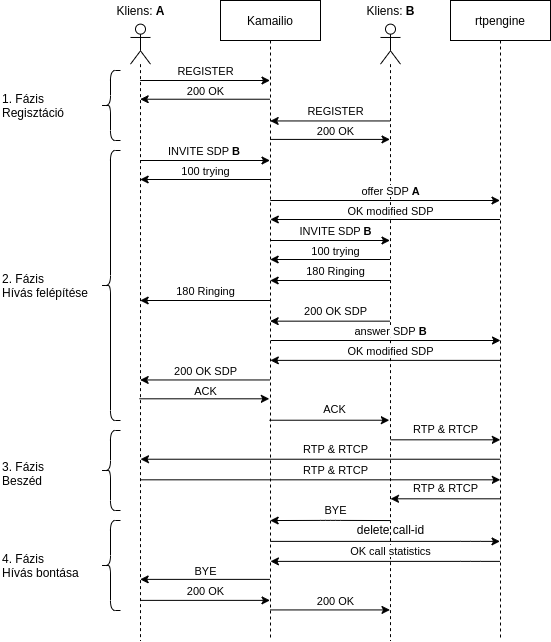
\includegraphics[width=0.9\textwidth, keepaspectratio]{figures/basic_call_flow.png}
	\caption{Kubernetes nélküli hívásfelépítés}
	\label{fig:callflow}
\end{figure}

Az \ref{fig:callflow} ábra segítségével ismertetem a hívásfelépítés részeit.  Az ábrán 
látható egy teljes hívás folyamata a regisztrációtól egészen a hívás bontásáig. Négy 
részre bontottam a hívást annak érdekében, hogy könnyebb legyen a megértése.

Az első rész a regisztráció, amelynek során a felhasználók csatlakoznak a SIP szerverhez.
Ilyenkor a kliens \texttt{SIP REGISTER} üzenetet küld a szervernek, amikkel hozzáadni, 
törölni és lekérdezni lehet a felhasználó adait szerverről. Ha létezik a felhasználónak 
fiókja a szerveren, viszont még nem jelentkeztek be az adott eszközről akkor az első 
alkalommal egy \texttt{401 Unauthorized} üzenettel tér vissza, ami felszólítja a klienst, 
hogy adja meg a hitelesítéshez szükséges felhasználói azonosítót és jelszót, amit egy 
újabb \texttt{SIP REGISTER} üzenetben fog újraküldeni titkosítva. Ha minden megfelelt, 
akkor \texttt{200 OK} üzenetet kap vissza a kliens, ami jelzi, hogy minden rendben és tud 
hívásokat kezdeményezni. Az ábrán szereplő folyamat nem tartalmazza a \texttt{401} 
státusz üzenetet, mert már többször használva volt a kliens azon a virtuális gépen.

A következő rész pedig már a konkrét hívás kezdeményezése és felépítése. A hívást az 
\textbf{A} felhasználó kezdeményezi \textbf{B} irányába egy \texttt{INVITE} üzenettel, 
ami tartalmaz egy SDP üzenetet is. Ez az SDP egy olyan protokoll, amivel a híváshoz 
kapcsolódó információkat lehet továbbítani, mint például a támogatott média formátumok 
listája illetve a hívott fél elérhetőségei. Mivel ebben az esetben \textbf{B} felhasználó 
címe létezik a szerveren így a szerver \texttt{100 trying} üzenettel jelzi 
\textbf{A}-nak, hogy elkezdte a hívást felépíteni. Erre azért van szükség, hogy a kliens 
ne próbálkozzon újra a hívás felépítésével.

A szerver ilyenkor küld egy \texttt{offer} üzenetet az rtpengine felé, aminek legalább 
tartalmaznia kell az \textbf{A} által küldött SDP üzenetet, hívásazonosítót és a SIP 
üzenet \texttt{From} mezőjét, ami az \textbf{A} azonosítója. Erre az rtpengine egy 
módosított SDP üzenetet küld vissza a szervernek, amiben módosítja a cél címet és portot 
a sajátjára. Ezáltal minden RTP üzenet elsőnek az rtpengine-hez fog elmenni és majd onnét 
megy tovább \textbf{B}-nek.

Ha ez is sikeresen megtörtént, a szerver átveszi a hívás kezdeményező szerepét a 
\textbf{B}-vel szemben. Szóval küld egy \texttt{INVITE} üzenetet neki, amiben szerepel 
\textbf{A} azonosítója, de a csatlakozást leíró mező az rtpengine címe lesz. A 
\texttt{trying} üzenet ebben az esetben is ugyan azt jelenti, mint mikor az \textbf{A} 
kezdeményezett. De itt már szerepel a \texttt{180 ringing}, amivel lehet jelzi, hogy 
feldolgozásra került az \texttt{INVITE}. Majd ugyan ez az üzenetet megkapja \textbf{A} 
is. 

Ha \textbf{B} elfogadta a hívást, akkor \texttt{200 OK} státusszal jelez a szervernek, 
amiből a SIP szerver tudja, hogy \texttt{answer}-t kell küldenie az rtpengine felé, 
amivel a hívás teljesen ki fog épülni az rtpengine-ben is. Az \texttt{answer} igazából 
ugyanazt a funkciót valósítja meg, mint az \texttt{offer}. Mivel az rtpengine kapott 
\texttt{offer}-t és \texttt{answer}-t is, így a hívást kiépítheti és az előzőleg 
lefoglalt négy porton képes fogadni a forgalmat, amit feldolgozva tovább küld. Azért 
foglal le négy port, mert felenként kell egy páros számú port az RTP forgalomnak és egy 
páratlan számú az RTCP-nek. Végül pedig egy \texttt{SIP ACK} üzenettel van értesítve mind 
a két fél arról, hogy a hívás sikeresen kiépült és elkezdhetnek beszélni. 

Mivel már létezik a hívás, lehet küldeni a forgalmat az rtpengine adott 
portjaira. Ahol a legegyszerűbb esetben annyi történik, hogy az \textbf{A}-hoz rendelt
RTP porton kapott csomagokat kiküldi a \textbf{B}-hez a hozzárendelt portról. Ugyanez
történik RTCP esetében is. 

Mikor vége a hívásnak, akkor megkezdődik a hívás lebontása egy \texttt{BYE SIP} 
üzenettel. Aminek hatására a SIP szerver egy \texttt{delete} üzenetet ad ki az rtpengine 
felé, ami tartalmazza a hívás azonosítóját. Ekkor törlődik minden a híváshoz kapcsolódó 
információ és a számukra kinyitott portok is lezárnak. De a rtpengine válaszában 
szerepelnek a hívásról információk, amik alapján könnyen lehet statisztikákat készíteni 
például a hívások átlagos hosszáról vagy minőségéről.